\documentclass[dvipsnames,tikz]{standalone}
\usepackage{amsmath}
\usepackage{xcolor}
\usepackage{tikz}
\usetikzlibrary{calc}
\usetikzlibrary{decorations.pathreplacing,calligraphy,3d}


\begin{document}
	% add color=white for dark mode
	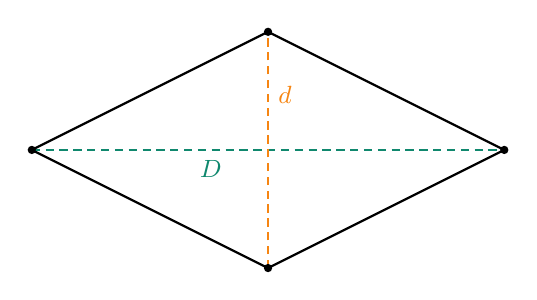
\begin{tikzpicture}[thick, color=black] 
		\draw (0,0) -- (3,-1.5) -- (6,0) -- (3,1.5) -- cycle;
		\draw[densely dashed, PineGreen] (0,0) -- (6,0);
		\draw[densely dashed, BurntOrange] (3,-1.5) -- (3,1.5);
		
		
		\begin{scope}[font=\small]
			\fill (0,0) circle (1.5pt);
			\fill (6,0) circle (1.5pt);
			\fill (3,1.5) circle (1.5pt);
			\fill (3,-1.5) circle (1.5pt);
			\draw[PineGreen] (3,0) node [below left, xshift=-13pt] {$D$};
			\draw[BurntOrange] (3,0) node [above right, yshift=13pt] {$d$};
		\end{scope}
	\end{tikzpicture} 
	
\end{document}